\section{Riemann and the Reinvention of Integration (1854)}

\subsection{After Cauchy: Cleaning Up Infinity, One Sum at a Time}

Cauchy had patched the cracks in calculus. He gave us rigorous limits, continuity, and differentiability. But there was still one place where the old ghosts of infinitesimals lingered: \textbf{integration}.

Sure, mathematicians could differentiate with rigor now. But integration still leaned on old metaphors—“summing infinitely many infinitesimal slices” sounded poetic, but it wasn’t clear what that really meant.

What did it mean to add up infinitely many values?

How could an infinite sum produce a finite area?

And most awkward of all: \textbf{what counts as an “area” when the function keeps misbehaving?}

For smooth, well-behaved functions, nobody worried. But as analysis matured, mathematicians were no longer content with “functions that played nice.” Fourier had already shown that useful functions—like square waves and discontinuous signals—refused to stay smooth. And if mathematics was going to handle the messy, the jagged, the discontinuous, it needed a new kind of integral.

That’s where \textbf{Bernhard Riemann} stepped in.

He wasn’t just solving technicalities. He was answering a deeper question:

\begin{center}
\emph{How do you measure area when the curve won’t cooperate?}
\end{center}

Riemann’s answer? Don’t start with infinitesimals—start with \textbf{finite sums}, then make them \textbf{converge}.

And in doing so, he reinvented integration.

\subsection{Riemann Sums: Approximating Area Through Partitions}

Riemann’s key insight was that the \textbf{integral of a function over an interval} could be understood as the limit of finite sums of function values over smaller and smaller partitions of that interval.  

Mathematically, he defined the \textbf{Riemann sum} as:  

\[
S = \sum_{i=1}^{n} f(x_i^*) \Delta x_i
\]

where:  
\begin{itemize}
    \item The interval \([a, b]\) is divided into \textbf{subintervals} \([x_{i-1}, x_i]\), each of width \( \Delta x_i = x_i - x_{i-1} \).  
    \item A representative sample point \( x_i^* \) is chosen from each subinterval.  
    \item The function value at \( x_i^* \) is multiplied by the subinterval width to approximate the area of each strip.  
\end{itemize}

\begin{center}
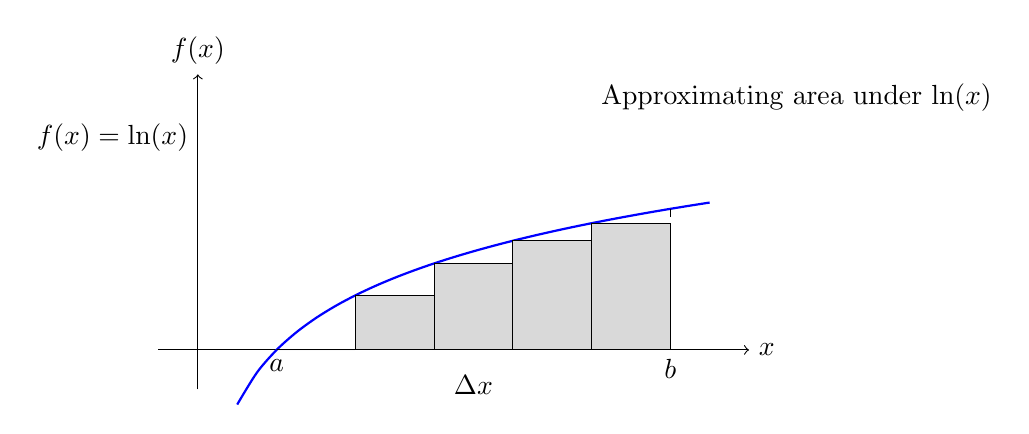
\begin{tikzpicture}
    % Draw axes
    \draw[->] (-0.5,0) -- (7,0) node[right] {\( x \)};
    \draw[->] (0,-0.5) -- (0,3.5) node[above] {\( f(x) \)};
    
    % Function curve: natural logarithm
    \draw[thick, blue, domain=0.5:6.5, smooth] plot (\x, {ln(\x)});
    
    % Interval [a, b]
    \node[below] at (1,0) {\( a \)};
    \node[below] at (6,0) {\( b \)};
    
    % Vertical dashed lines for subintervals
    \foreach \x in {1,2,3,4,5,6} {
        \draw[dashed] (\x,0) -- (\x,{ln(\x)});
    }

    % Rectangles (Riemann sum representation)
    \foreach \x in {1,2,3,4,5} {
        \pgfmathsetmacro\height{ln(\x)}
        \draw[fill=gray!30] (\x,0) rectangle (\x+1,\height);
    }

    % Labels
    \node[below] at (3.5,-0.2) {\( \Delta x \)};
    \node[left] at (0,2.7) {\( f(x) = \ln(x) \)};
    
    % Text description
    \node[right] at (5,3.2) {Approximating area under \( \ln(x) \)};
\end{tikzpicture}
\end{center}


By taking the \textbf{limit as the number of subintervals approaches infinity} (while the width of each subinterval shrinks to zero), the sum converges to a well-defined value—this is the \textbf{Riemann integral}:  

\[
\int_a^b f(x) \,dx = \lim_{n \to \infty} \sum_{i=1}^{n} f(x_i^*) \Delta x_i
\]

This formalization replaced the vague notion of “summing infinitely small quantities” with a \textbf{clear limit process}, ensuring that integration was built on the same solid foundations as differentiation.  







\begin{figure}[H]
\centering
\begin{tikzpicture}
\matrix[matrix of nodes, column sep=1.2cm, row sep=1.2cm] {
% Top-left: 2 rectangles
\node {
  \begin{tikzpicture}[scale=0.6]
    \draw[->] (-0.5,0) -- (7,0) node[right] {\(x\)};
    \draw[->] (0,-0.5) -- (0,3.5) node[above] {\(f(x)\)};
    \draw[thick, blue, domain=1:6.2, smooth] plot (\x, {ln(\x)});
    \foreach \x in {1,3.5} {
        \pgfmathsetmacro\h{ln(\x)}
        \draw[fill=gray!30] (\x,0) rectangle ({\x+2.5}, \h);
    }
    \node at (3,-0.8) {\scriptsize 2 rectangles};
  \end{tikzpicture}
}; &
% Top-right: 3 rectangles
\node {
  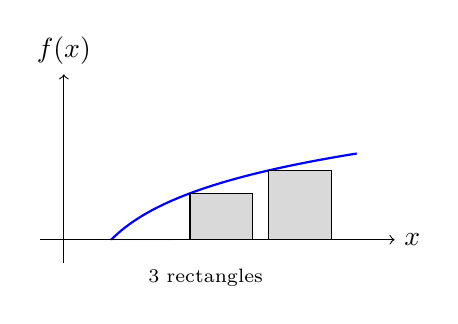
\begin{tikzpicture}[scale=0.6]
    \draw[->] (-0.5,0) -- (7,0) node[right] {\(x\)};
    \draw[->] (0,-0.5) -- (0,3.5) node[above] {\(f(x)\)};
    \draw[thick, blue, domain=1:6.2, smooth] plot (\x, {ln(\x)});
    \foreach \x in {1,2.67,4.33} {
        \pgfmathsetmacro\h{ln(\x)}
        \draw[fill=gray!30] (\x,0) rectangle ({\x+1.33}, \h);
    }
    \node at (3,-0.8) {\scriptsize 3 rectangles};
  \end{tikzpicture}
}; \\
% Bottom-left: 5 rectangles
\node {
  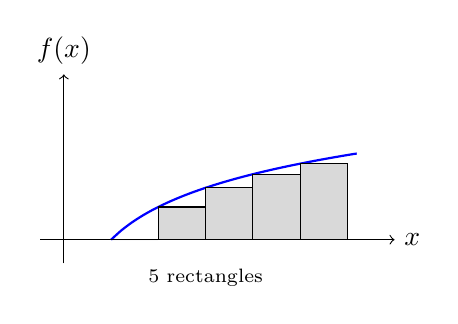
\begin{tikzpicture}[scale=0.6]
    \draw[->] (-0.5,0) -- (7,0) node[right] {\(x\)};
    \draw[->] (0,-0.5) -- (0,3.5) node[above] {\(f(x)\)};
    \draw[thick, blue, domain=1:6.2, smooth] plot (\x, {ln(\x)});
    \foreach \x in {1,2,3,4,5} {
        \pgfmathsetmacro\h{ln(\x)}
        \draw[fill=gray!30] (\x,0) rectangle ({\x+1}, \h);
    }
    \node at (3,-0.8) {\scriptsize 5 rectangles};
  \end{tikzpicture}
}; &
% Bottom-right: 10 rectangles
\node {
  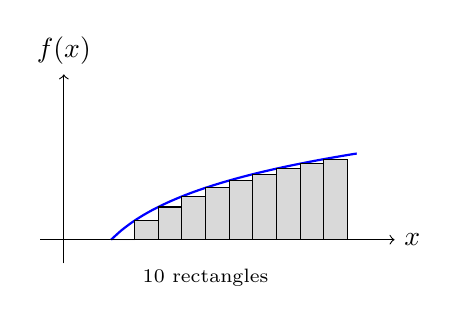
\begin{tikzpicture}[scale=0.6]
    \draw[->] (-0.5,0) -- (7,0) node[right] {\(x\)};
    \draw[->] (0,-0.5) -- (0,3.5) node[above] {\(f(x)\)};
    \draw[thick, blue, domain=1:6.2, smooth] plot (\x, {ln(\x)});
    \foreach \x in {1,1.5,...,5.5} {
        \pgfmathsetmacro\h{ln(\x)}
        \draw[fill=gray!30] (\x,0) rectangle ({\x+0.5}, \h);
    }
    \node at (3,-0.8) {\scriptsize 10 rectangles};
  \end{tikzpicture}
}; \\
};
\end{tikzpicture}
\caption{Left-endpoint Riemann sums: as the number of rectangles increases, the approximation of the area under \( \ln(x) \) becomes more accurate.}
\end{figure}

\subsection{When Even Riemann Fails: The Dirichlet Function Arrives}

Riemann’s definition of the integral was a triumph of mathematical structure—a way to make sense of wildly misbehaving functions that still held some local order. Where Fourier had cracked open the world of discontinuities, Riemann offered a way to clean up the mess—at least for most of them.

But then came the Dirichlet function.

If the square wave was a rebellious teen testing the limits of classical analysis, the Dirichlet function was a full-blown existential threat.

\[
f_{\text{Dirichlet}}(x) =
\begin{cases}
1, & x \in \mathbb{Q} \\
0, & x \in \mathbb{R} \setminus \mathbb{Q}
\end{cases}
\]

This function is discontinuous \emph{everywhere}. There’s no interval, no neighborhood, no zoom level at which it behaves. It doesn’t spike—it flickers. Rational numbers, being dense, are always nearby. So are irrationals. No matter how small your partition, you’re trapped in a blur of ones and zeros.

And that’s the problem.

Riemann’s method relies on refining partitions: slicing up the interval, choosing representative points, and watching the sums converge. But with the Dirichlet function, there’s no “good” point to pick. Every subinterval is chaos in miniature. Every choice of \(x_i^*\) gives a different answer, and none of them stabilize. The limit simply doesn’t exist.

\begin{quote}
It’s not that the function resists integration.  
It refuses to even be approximated.
\end{quote}

This wasn’t just a mathematical curiosity—it was a full-blown philosophical crisis. The Dirichlet function didn’t just break Riemann’s method; it broke the illusion that all functions could be tamed by clever definitions.

It forced mathematicians to confront an uncomfortable truth:  
not all functions are integrable—even with Riemann’s rigor.

\medskip

And worse: this wasn't the last such function. The 19th century would soon turn into a parade of pathological examples—functions continuous everywhere but differentiable nowhere, limits of convergent series that behaved like statistical hallucinations.

\begin{quote}
Riemann had built a sturdy floor beneath calculus.  
But the Dirichlet function was a trapdoor.
\end{quote}

Soon, someone would open it—and drop us into the abyss.



\subsection{When Riemann Breaks: The Crisis of Convergence}

Riemann had rescued integration. By replacing the vague idea of “infinitely small quantities” with a rigorous limit of sums over partitions, he made the integral precise, predictable, and powerful.

But as mathematics often does, it asked the next uncomfortable question:

\begin{center}
\emph{What happens when even Riemann's rigor isn't enough?}
\end{center}

For all its elegance, the Riemann integral depends on a kind of behavioral decency: that a function behaves “well enough” over small intervals for its sum to stabilize. If we can slice an interval into thinner and thinner subintervals, evaluate the function on each, and let those values add up to something meaningful—great. That’s the integral.

But then came the rebels. Functions that refused to play nice.

These weren’t just sharp or spiky—they were unruly in a deeper sense. On every subinterval, no matter how small, the function could jump, flip, or oscillate without warning. The idea of convergence—the soul of the Riemann sum—evaporated. Sums didn’t stabilize. They danced. They defied reason.

\medskip

This wasn’t just a technicality—it was a philosophical blow.

If integration is supposed to measure “area,” then some functions made measurement meaningless. The more you tried to pin them down, the more they slipped through your fingers. Refining the partition no longer improved the approximation—it just revealed more chaos.

\begin{quote}
The Dirichlet function, for example, was like trying to measure fog with a ruler.
\end{quote}

It forced mathematicians to confront a terrifying possibility:

\begin{center}
\emph{What if not all functions are measurable—not even in Riemann’s sense?}
\end{center}

Mathematics had finally caught up to the implications of its own creations. Fourier had opened the door to infinite decomposition. Riemann tried to contain the madness. But lurking just beyond that containment was something worse: the realization that continuity, reason, and even area could all fail—simultaneously.

\medskip

This wasn’t the end of analysis.

But it was the beginning of a reckoning.

Soon, others would take the stage—not just to refine Riemann’s ideas, but to question everything beneath them. One in particular would detonate what little intuition remained about “smoothness” and “functions.” His name? Let’s just say: you’ll know a monster when you meet one.
